\documentclass[11pt]{article}
\usepackage{array,booktabs,arydshln,xcolor}
\usepackage{tikz}
\usetikzlibrary{arrows}
\usetikzlibrary{patterns.meta}
\usetikzlibrary{decorations.pathreplacing}
\usetikzlibrary{decorations.markings,fpu}
\usetikzlibrary{decorations.pathmorphing}
\usepackage{amsmath}

\newcommand{\e}{\varepsilon}

\begin{document}

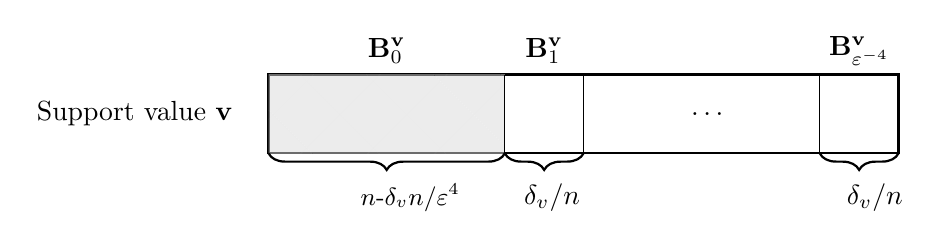
\begin{tikzpicture}
\pgfmathtruncatemacro{\totalL}{8};
\pgfmathtruncatemacro{\step}{1};
\pgfmathtruncatemacro{\blockZero}{3};

\pgfmathtruncatemacro{\height}{1};

%Draw rectangle
\draw [draw=black, thick] (0,0) rectangle (\totalL,\height);

%Draw blocks' limits
%block 0
%Fill shapes with color
\fill[pattern={Lines[angle=45, distance=6mm, line width=13mm, xshift=5mm]}, pattern color=gray!30,opacity=.5] ((0,0)--(\blockZero,0)--(\blockZero,\height)--(0,\height)--(0,0);

\draw[-] (\blockZero,0) -- (\blockZero,\height) ;

%Block 1
\draw[-] (\step+\blockZero,0) -- (\step+\blockZero,\height) ;

%Block 2
\draw[-] (\totalL-\step,0) -- (\totalL-\step,\height) ;

\node[] at (-1.7*\step, 0.5*\height) {Support value $\mathbf{v}$};

%Draw blocks nodes
\node[] at (0.5*\blockZero, 1.3*\height) {$\mathbf{B}_0^\mathbf{v}$};

\node[] at (0.5*\step+\blockZero, 1.3*\height) {$\mathbf{B}_1^\mathbf{v}$};

\node[] at (0.7*\totalL,0.5*\height) {$\dots$};

\node[] at (\totalL-0.5*\step, 1.3*\height) {$\mathbf{B}_{\e^{-4}}^\mathbf{v}$};

%Draw braces
\draw [decorate,black,thick,decoration={brace,amplitude=6pt, mirror}] (0,0) -- (\blockZero,0) node[label={[xshift=-1.2cm, yshift=-1cm]{\small $n\text{-}\delta_v n/\e^4$}}]{};

\draw [decorate,black,thick,decoration={brace,amplitude=6pt, mirror}] (\blockZero,0) -- (\blockZero+\step,0) node[label={[xshift=-0.4cm, yshift=-1cm]$\delta_v/n$}]{};

\draw [decorate,black,thick,decoration={brace,amplitude=6pt, mirror}] (\totalL-\step,0) -- (\totalL,0) node[label={[xshift=-0.3cm, yshift=-1cm]$\delta_v/n$}]{};


\end{tikzpicture}

\end{document}